\chapter{Gaussian Processes}

\begin{itemize}
    \item Prove all pos-sem is cov
    \item expand on intro to motive the section
    \item prove exponential quad kern is pos semi-def
\end{itemize}

\section{Motivation and Preliminaries}

Fundamentally, approximate Bayesian computation is a form of Monte Carlo
integration, where sampling a discrepancy is sampling from the discrepancy
distribution at a given parameter. If we knew the distribution of the
discrepency function exactly, then in order to do approximate
Bayesian computation, we would not need to actually run the model in order to
obtain a `sample' discrepency. Instead we could draw from the distribution of the
discrepency function for a fixed $\bm\theta.$ Further, since acceptance
rejection sampling from our discrepency function approximates something
proportional to the likelihood, if our discrepency function approximation is
close to the actual distribution of the discrepency, we can create an excplicit
synthetic approximate likelihood $\LABC(\bm\theta)\propto \mathcal{L}(\theta)$
and use this directly to obtain posterior samples, or even just find maximimum
likelihood estimates.

To do this, we make the assumptions $\mu(\bm\theta) = \E(D(\bm\theta))$
(or $\E[\ln(D(\bm\theta))] = \mu(\bm\theta)$) is
continuous in theta, $\mathrm{var}(D(\bm\theta)) = \sigma^2_o$
(or $\mathrm{var}[\ln(D(\bm\theta))] = \sigma^2_o$) constant for all theta,
and $D(\bm\theta) \sim N(\mu(\bm\theta), \sigma^2_o)$ for fixed $\bm\theta.$

We consider a class of plausible functions for $\mu(\bm\theta)$, and assign
some underlying prior
probability to each of them. We can then directly simulate from our model to
return a discrepency for a fixed $\bm\theta$ that updates the probability of
each function being the `true' $\mu(\bm\theta)$
function. The class of function we consider are those generated by Gaussian
processes. \textcolor{red}{
    Further discussion on the `distribution' of Gaussian processes on an
    uncountably infinite support is in the appendices.
}

\begin{definition}[Gaussian Process]\label{def:gp}
    A collection of random variables $\{f(x)\}_{x\in\mathcal{X}}$
    (where $x$ may be a vector) is a \emph{Gaussian process} if any finite
    subset of the collection of random variables is multivariate normal
    distributed. That is, there is a function $m:\mathcal{X}\to\R$ and
    symmetric kernel $k:\mathcal{X}\times\mathcal{X}\to \R$ such that for all
    finite sets
    $\mathbf{x} :=\{x_1, x_2, \dots, x_n\} \subset \mathcal{J},$ with
    $f(\mathbf{x}) := [f(x_1), f(x_2), \dots, f(x_n)]^T$
    $$f(\mathbf{x}) \sim
        \MVN\left(\begin{bmatrix}
            m(x_1) \\ m(x_2)\\ \vdots\\ m(x_n)
        \end{bmatrix},\, \mathbf{K} = \begin{bmatrix}
            k(x_1, x_1) & k(x_1, x_2) & \dots  & k(x_1, x_n) \\
            k(x_2, x_1) & \ddots      &        & \vdots      \\
            \vdots      &             & \ddots & \vdots      \\
            k(x_n, x_1) & \cdots      & \cdots & k(x_n, x_n)
        \end{bmatrix}\right).$$
\end{definition}

\begin{definition}[Mean and Covariance Function]\label{def:mean_kernel}
    We define the \emph{mean function} and \emph{covariance kernels} as
    $$m(x_i) := \E\left[f(x_i)\right]$$ and
    $$k(x_{i}, x_{i^\prime}) := \cov\left(f(x_i), f(x_{i^\prime})\right).$$
\end{definition}

For the rest of the discussion, we assume $m \equiv 0,$ but there will be a
brief discussion on non-zero mean functions. Although on $\R^d$ Gaussian
processes are a collection of (uncountably infinite)
random variables, we consider kernels such that
$\mathrm{corr}(x, x^\prime) \to 1$ as $||x - x^\prime||\to 0$ for some norm,
all realisations of the Gaussian process will be continuous in $x$ almost
surely, hence we can consider these as realisations of continuous functions.
\textcolor{red}{(Should I prove this?)}

Some common examples of Gaussian processes include \begin{enumerate}
    \item Brownian motion on $\R$:
          $$m\equiv 0, \quad \text{and}\quad k(s, t) = \min(s, t)$$
    \item Ornstein Uhlenbeck process with parameters $\theta$ and $\sigma$:
          $$
              m\equiv 0, \quad \text{and}
              \quad k(s, t)
              = \frac{\sigma^2_k}{2\theta} \left(
              e^{-\theta|t - s|} - e^{-\theta(t + s)}
              \right)
          $$
\end{enumerate}

% \begin{definition}[Brownian Motion]
%     $B(t):\R^+ \to \R$ is a \emph{Brownian motion} on $\R$ if\begin{enumerate}
%         \item $B(0) = 0$ almost surely
%         \item $B(t_0), B(t_1) - B(t_0), \dots, B(t_n - t_{n-1})$ are
%               independent for all $t_0<t_1<t_2<\dots<t_n$
%         \item $B(t + s) - B(t)\sim N(0, s)$ for $s, t \geq 0$
%         \item $B(t)$ is continuous almost surely for $t>0.$
%     \end{enumerate}
% \end{definition}

The properties (such as smoothness and rate of fluctuation) of the
realised functions are determined by the class
covariance kernel $k,$ as well as any related hyperparameters. Before exploring
different kernel options, we begin by
\textcolor{red}{defining a valid kernel function, and} formalising `smoothness.'

\color{red}

\begin{definition}[Positive Semi-Definite Matrix]\label{def:pos_def_mat}
    An $n\times n$ matrix $\mathbf{A}$ is \emph{positive semi-definite} if
    $\mathbf{v}^T\mathbf{A}\mathbf{v} \geq 0$ for all $\mathbf{v}\in\R^n.$
\end{definition}

\begin{theorem}[Sufficient Condition for Positive Semi-Definite]
    A symmetric matrix $\mathbf{A}$ is positive semi-definite, if (and only if)
    it's eigenvalues are non-negative.
\end{theorem}
\begin{proof}
    % https://en.wikipedia.org/wiki/Definite_matrix#Eigenvalues
\end{proof}

\begin{definition}[Positive Semi-Definite Kernel]\label{def:pos_def_ker}
    A kernel $k:\mathcal{X}\times\mathcal{X}\to\R$ is
    \emph{positive semi-definite} if the matrix
    $$\mathbf{K} = \begin{bmatrix}
            k(x_1, x_1) & k(x_1, x_2) & \dots  & k(x_1, x_n) \\
            k(x_2, x_1) & \ddots      &        & \vdots      \\
            \vdots      &             & \ddots & \vdots      \\
            k(x_n, x_1) & \cdots      & \cdots & k(x_n, x_n)
        \end{bmatrix}$$
    is positive semi-definite for any collection of $x_i\in\mathcal{X}$
\end{definition}

\begin{theorem}
    All symmetric positive semi-definite matrices are covariance matrices for
    some set of random variables
\end{theorem}
\begin{proof}
    % https://www.fepress.org/wp-content/uploads/2014/06/ch7-iff-covariance_correlation_matrix.pdf
\end{proof}

\color{black}

\begin{definition}[Mean Square Continuous]
    A function $f:\R^d\to\R$ is \emph{mean square continuous} at $\mathbf{x}$
    in the $i$th direction at if
    $\E(|f(\mathbf{x} + h\mathbf{e}_i) - f(\mathbf{x})|^2)\to 0$ as $|h|\to 0,$
    where $\mathbf{e}_i$ is the unit vector with a 1 in the $i$th coordinate.
\end{definition}

\begin{definition}[Mean Square Differentiable]
    A function $f:\R^d\to\R$ is \emph{mean square differentiable} at
    $\mathbf{x}$ in the $i$th direction with derivative
    $\frac{\partial f(\mathbf{x})}{\partial x_i}$ if
    $$
        \E\left[
            \left|
            \frac{f(\mathbf{x} + h\mathbf{e}_i) - f(\mathbf{x})}{h}
            - \frac{\partial f(\mathbf{x})}{\partial x_i}
            \right|^2
            \right]\to 0
    $$ as $|h|\to 0,$ where $\mathbf{e}_i$ is the unit vector in the direction
    of the $i$th coordinate.
\end{definition}

The concept of mean square differentiability and continuity are analogous to
differentiability and continuity in the non-random function case.

\begin{theorem}
    Brownian motion is mean square continuous, but not mean square
    differentiable.
\end{theorem}
\begin{proof}
    $(B_{t + h} - B_t)^2 \sim (\sqrt{|h|}Z)^2$ where $Z\sim N(0,1).$ Therefore
    $(B_{t + h} - B_t)^2 \sim |h|\chi_1^2 \to 0$ almost surely as $|h|\to 0,$
    and hence $\E[(B_{t + h} - B_t)^2= 0]$. Since
    $\frac{B_{t + h} - B_t}{h} \sim N(0, 1/|h|),$ $\frac{B_{t + h} - B_t}{h}$
    does not converge to any valid probability distribution as $|h| \to 0,$ as
    the variance approaches $+\infty.$
\end{proof}

Some common

\color{red}

\begin{theorem}[Positive Semi-Definiteness of RBF]\label{thm:rbf_pos_def}
    The radial basis function
    ${\sigma^2_k}\exp(-\frac{(x - x^\prime)^2}{2\gamma^2})$ is a positive
    semi-definite kernel.
\end{theorem}

\begin{theorem}[Bochner's Theorem]
    Let $k$ be a stationary kernel function such that
    $k(x, x^\prime) = f(d)$. A function $k:\R^d\to\mathbb{C}$ is the covariance
    function of a weakly
    stationary mean square continuous complex-valued random process of $\R^d$
    if and only if it can be represented as
    $$k(\mathbf{\tau}) = \int_{\R^d} \exp(2\pi i \mathbf{s}\cdot\mathbf{\tau})$$
\end{theorem}

\parencite[82]{rasmussen_gaussian_2008}

\color{black}

\section{Classes of Kernel Function}

\subsection*{Mat\'{e}rn Class}

The Mat\'ern class of kernel gives flexibility over how many times mean square
differentiable the realised function is.

The Mat\'ern exponential kernel is of the form
$$k_\nu(x, x^\prime)
    = \sigma^2_k \frac{2^{1 - \nu}}{\Gamma(\nu)}
    \left(\frac{\sqrt{2\nu}||x - x^\prime||}{\ell}\right)^\nu
    K_\nu\left(-\frac{\sqrt{2\nu}||x - x^\prime||}{\ell}\right)$$
where $K_\nu$ is a modified Bessel function
(defined in \cite[374]{abramowitz_handbook_2013}). The general form is not very
insightful, however for $\nu = 1/2, 3/2$ and $5/2,$ the kernel
can be written as:
$$
    k_{1/2}(x, x^\prime)
    = \sigma^2_k\exp\left(-\frac{||x - x^\prime||}{\ell}\right)
$$
$$
    k_{3/2}(x, x^\prime)
    = \sigma^2_k
    \left(1 + \frac{\sqrt{3}||x - x^\prime||}{\ell}\right)
    \exp\left(-\frac{\sqrt{3}||x - x^\prime||}{\ell}\right)
$$
$$
    k_{5/2}(x, x^\prime)
    = \sigma^2_k
    \left(
    1 + \frac{\sqrt{5}||x - x^\prime||}{\ell} + \frac{5||x - x^\prime||}{3\ell^2}
    \right)
    \exp\left(-\frac{||x - x^\prime||^2}{2*\ell^2}\right)
$$

\begin{figure}[htbp]
    \centering
    \begin{subfigure}[b]{0.5\textwidth}
        \centering
        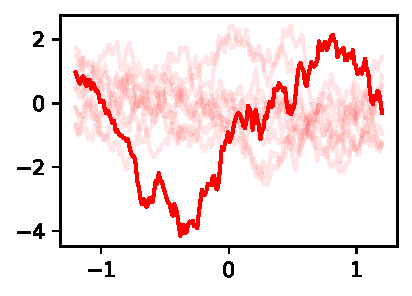
\includegraphics[width=\textwidth]{maternonehalf_kernel.pdf}
        \subcaption{Mat\'ern 1/2 Kernel}
        \label{fig:mat_one_half}
    \end{subfigure}%
    \hfill%
    \begin{subfigure}[b]{0.5\textwidth}
        \centering
        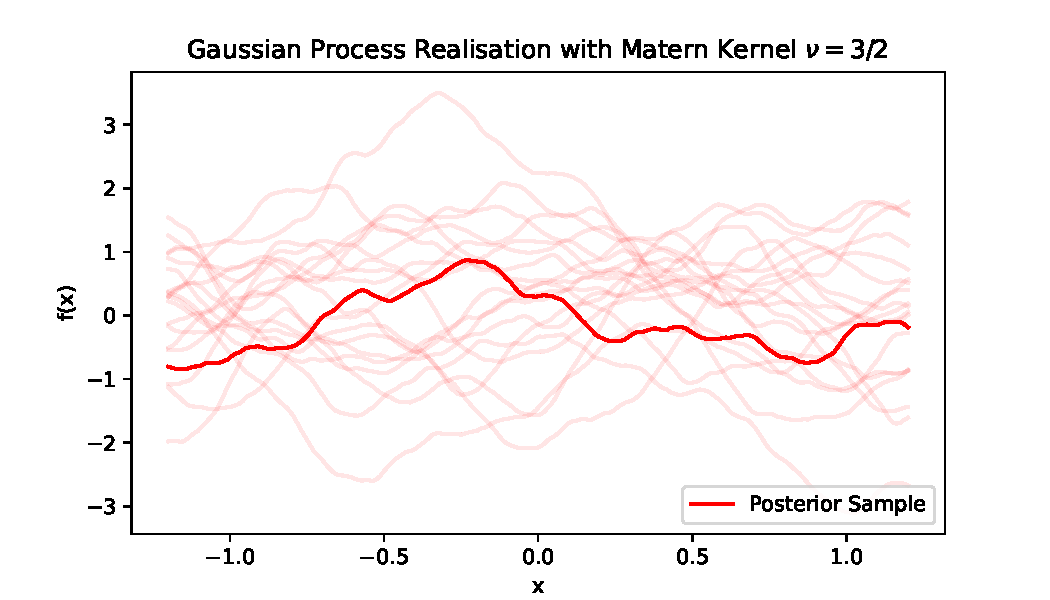
\includegraphics[width=\textwidth]{maternthreehalves_kernel.pdf}
        \subcaption{Mat\'ern 3/2 Kernel}
        \label{fig:mat_three_halves}
    \end{subfigure}
    \begin{subfigure}[b]{0.5\textwidth}
        \centering
        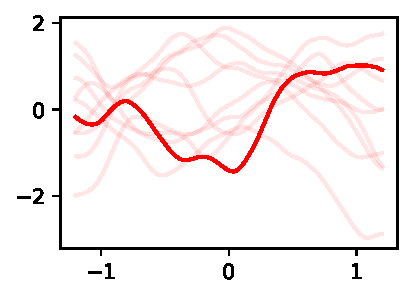
\includegraphics[width=\textwidth]{maternfivehalves_kernel.pdf}
        \subcaption{Mat\'ern 5/2 Kernel}
        \label{fig:mat_five_halves}
    \end{subfigure}%
    \hfill%
    \begin{subfigure}[b]{0.5\textwidth}
        \centering
        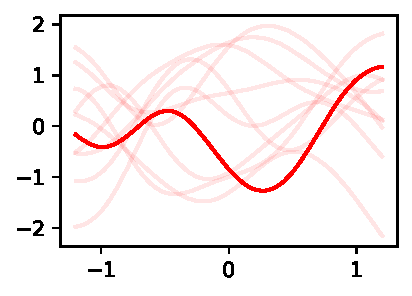
\includegraphics[width=\textwidth]{exponentiated_kernel.pdf}
        \subcaption{Squared Exponential Kernel}
        \label{fig:squared_exp}
    \end{subfigure}%
    \caption{
        Ten sample realisations from 4 different kernels with hyperparameters
        $\ell = 1,$ and $\sigma^2_o = 1.$ One realisation is bolded. Samples
        for each kernel were generated from the same seed.
    }
    \label{fig:kernels}
\end{figure}

Zero mean Gaussian processes with a Mat\'ern kernel are $n$ times mean square
differentiable, for all $n < \nu.$ This can be seen in Figure \ref{fig:kernels}
As $\nu\to\infty,$ with appropriate
rescaling, the limit of the Mat\'ern kernel is the squared exponential
kernel.\cite[85]{rasmussen_gaussian_2008}
\textcolor{red}{LOOK AT CHAPTER 4 SKOROKHOD STOCHASTIC I}

\subsection*{Squared Exponential}

The squared exponential kernel is of the form
$$
    k(x, x^\prime)
    = \sigma^2_k\exp\left(-\frac{||x - x^\prime||^2}{2\ell^2}\right)
$$

As the limit of Mat\'ern kernels, the squared exponential kernel is infinitely
mean square differentiable. Despite this being the `default' kernel in much of
the literature, infinite differentiability is a very strong condition on
functions which are very smooth, which can be seen in Figure
\ref{fig:squared_exp}

\subsection*{Choosing an Appropriate Kernel}

The appropriate choice of kernel will depend on the properties behaviour of the
target function to approximate. In the case of estimating an extremely
stochastic distribution (such as the price of a stock over time), it is
unlikely to be smooth, so no mean square differentiability is required, and a
Mat\'ern 1/2 kernel would be appropriate. If it is known that our target
function is extremely smooth, such as a finite sum of infinitely differentiable
functions (such as polynomials, sin, cos etc.) then the choice of squared
exponential kernel is the most appropriate kernel. Realistically, the
smoothness of the function will not be known a priori, and hence some sort of
compromise (such as Mat\'ern 5/2) kernel allows for flexibility.

Many other kernels exist that induce varying behaviours, such as periodic
kernels \textcolor{red}{find periodic kernel}, and non-stationary kernels
(where the covariance is dependent on $x$ and $x^\prime$, not just
$|x - x^\prime|$)
\textcolor{red}{have i defined stationary?}.

\subsection*{Length and Amplitude Hyperparameters}

\begin{figure}[htbp]
    \centering
    \begin{subfigure}[b]{0.5\textwidth}
        \centering
        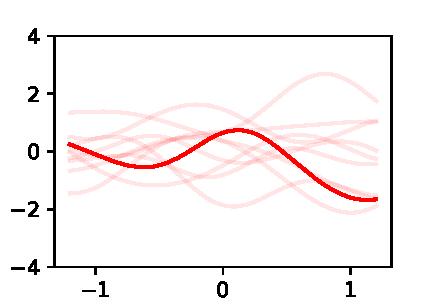
\includegraphics[width=\textwidth]{GP_ell_5_sigma2_5_tenths.pdf}
        \subcaption{$\ell = \sigma^2_k = 1/2$}
        \label{fig:half_half}
    \end{subfigure}%
    \hfill%
    \begin{subfigure}[b]{0.5\textwidth}
        \centering
        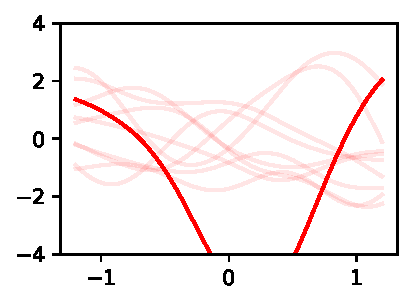
\includegraphics[width=\textwidth]{GP_ell_5_sigma2_20_tenths.pdf}
        \subcaption{$\ell = 1/2, \sigma^2_k = 2$}
        \label{fig:half_two}
    \end{subfigure}
    \begin{subfigure}[b]{0.5\textwidth}
        \centering
        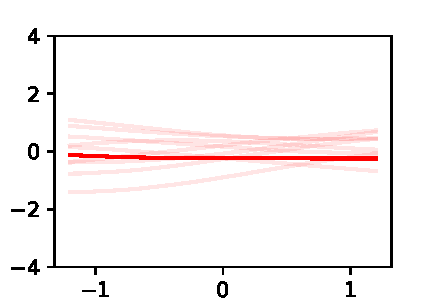
\includegraphics[width=\textwidth]{GP_ell_20_sigma2_5_tenths.pdf}
        \subcaption{$\ell = 2, \sigma^2_k = 1/2$}
        \label{fig:two_half}
    \end{subfigure}%
    \hfill%
    \begin{subfigure}[b]{0.5\textwidth}
        \centering
        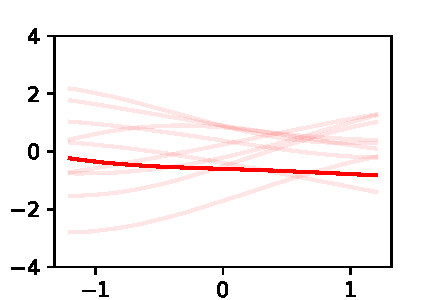
\includegraphics[width=\textwidth]{GP_ell_20_sigma2_20_tenths.pdf}
        \subcaption{$\ell = \sigma^2_k = 2$}
        \label{fig:two_two}
    \end{subfigure}%
    \caption{
        Ten realisations of zero mean Gaussian processes with the squared
        exponential kernel, varying the length and amplitude parameters.
        The samples were generated using the same seed
    }
    \label{fig:length_amp}
\end{figure}

In both the Mat\'ern and squared quadratic kernels
(as well as most other common kernels choices), there are two
hyperparameters $\ell$ and $\sigma^2_k$ which are referred to as length and
amplitude hyperparameters. $\ell$ determines how close two points need
to be to be highly correlated. Larger values of $\ell$ generates functions with
higher correlation within a larger neighbourhood,
as seen in Figure \ref{fig:length_amp}. $\sigma^2_k$ does not impact
the correlation between $x$ and $x^\prime,$ but scales the correlation
matrix. In other words, larger $\sigma^2_k$ increase the size but not rate of
fluctuations. This can be seen comparing Figure \ref{fig:half_half} to Figure
\ref{fig:half_two}.

\section{Gaussian Process Regression}

After choosing a set of prior distributions, given a set of observations, we
can condition our Gaussian process on these priors to update our distribution
of plausible functions. This is where beauty and simplicity in using Gaussian
processes shines through. A conditional multivariate normal distribution
is still multivariate normal, and so the distribution of unobserved points
reduces to elementary linear algebra.

Consider
$$
    \begin{bmatrix}
        f(\mathbf{x}_1) \\
        f(\mathbf{x}_2)
    \end{bmatrix} \sim \mathcal{N}\left(
    \begin{bmatrix}
            m(\mathbf{x}_1) \\
            m(\mathbf{x}_2)
        \end{bmatrix}, \begin{bmatrix}
            K_{11} & K_{12} \\
            K_{21} & K_{22}
        \end{bmatrix}
    \right)
$$
where $K_{ij} = \begin{bmatrix}
        k(x_{i1}, x_{j1})     & k(x_{i1}, x_{j2})     & \cdots & k(x_{i1}, x_{j{n_j}})     \\
        k(x_{i2}, x_{j1})     & k(x_{i2}, x_{j2})     & \cdots & k(x_{i2}, x_{j{n_j}})     \\
        \vdots                & \vdots                & \ddots & \vdots                    \\
        k(x_{i{n_i}}, x_{j1}) & k(x_{i{n_i}}, x_{j2}) & \cdots & k(x_{i{n_i}}, x_{j{n_j}})
    \end{bmatrix}$ if $\mathbf{x}_i$ is of length $n_i,$ and $\mathbf{x}_j$ is of length
length $n_j.$ Note that $K_{12} = K_{21}^T.$

$$
    f(\mathbf{x}_1) | f(\mathbf{x}_2)
    \sim \mathcal{N}\left(
    m(\mathbf{x}_1) + K_{12}K_{22}^{-1}(f(\mathbf{x}_2) - m(\mathbf{x}_2)), \,\,
    K_{11} - K_{12}K_{22}^{-1}K_{21}
    \right)
$$

\textcolor{red}{The proof is in the appendices.}

Therefore after observing the function at multiple indices, we update the
predictive distribution of any unobserved points as seen in Figure \ref{fig:no_var_cub_reg}

\begin{figure}[htbp]
    \centering
    \begin{subfigure}[b]{0.5\textwidth}
        \centering
        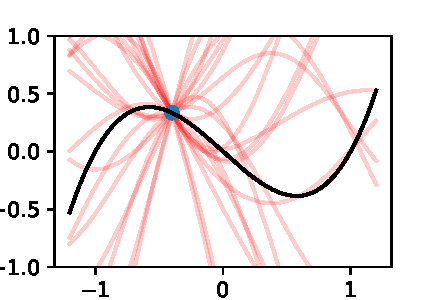
\includegraphics[width=\textwidth]{cub_GP_1_iters.pdf}
    \end{subfigure}%
    \hfill%
    \begin{subfigure}[b]{0.5\textwidth}
        \centering
        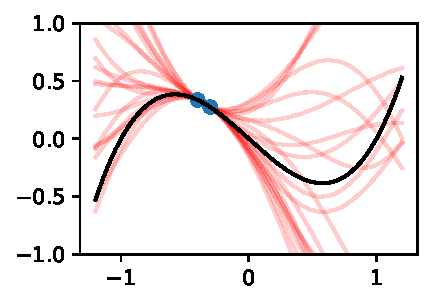
\includegraphics[width=\textwidth]{cub_GP_2_iters.pdf}
    \end{subfigure}
    \begin{subfigure}[b]{0.5\textwidth}
        \centering
        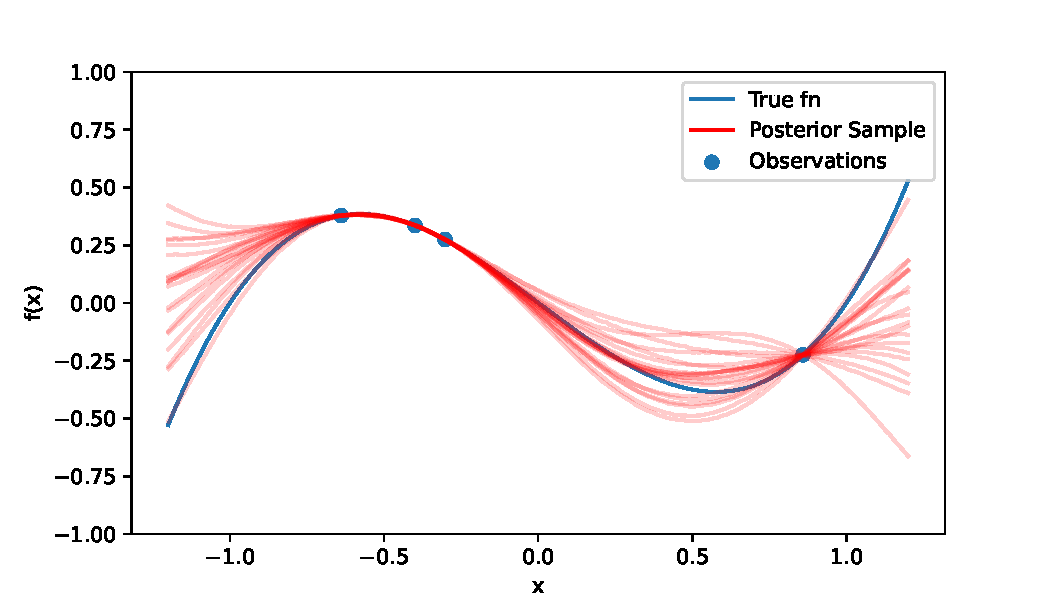
\includegraphics[width=\textwidth]{cub_GP_4_iters.pdf}
    \end{subfigure}%
    \hfill%
    \begin{subfigure}[b]{0.5\textwidth}
        \centering
        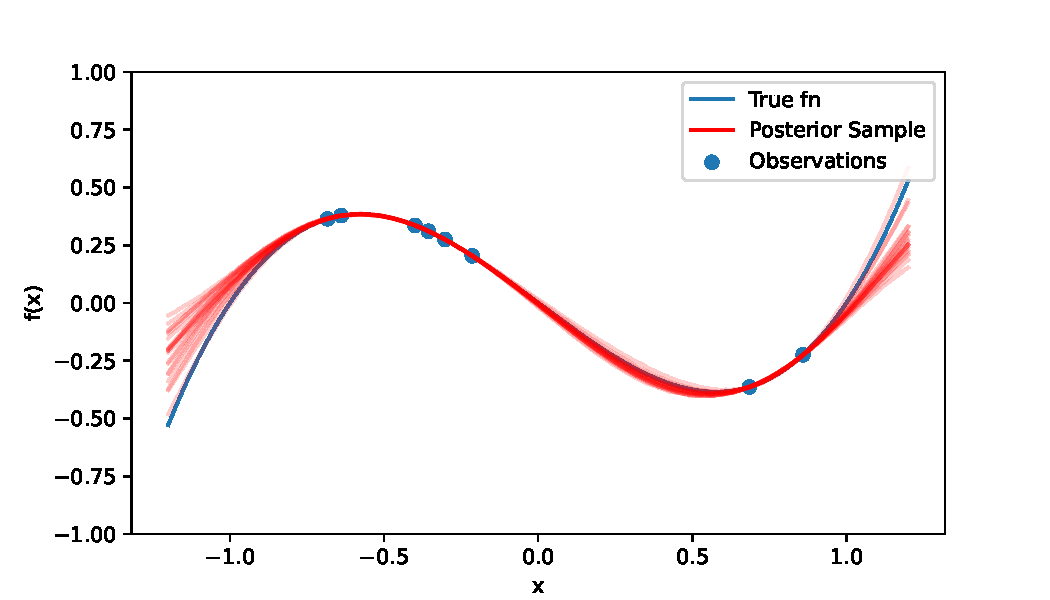
\includegraphics[width=\textwidth]{cub_GP_8_iters.pdf}
    \end{subfigure}%
    \caption{
        Sequence of Gaussian process regressions on the target function
        (black) $f(x) = x(x-1)(x+1),$ after 1, 2, 4, and 8 observations in
        blue. The red lines are new realisations from the conditioned Gaussian
        process. The Gaussian process was zero mean and had a squared
        exponential kernel. The hyperparameters were fixed with $\ell = 2.7$
        and $\sigma^2_k = 1.1$
    }
    \label{fig:no_var_cub_reg}
\end{figure}

\subsection*{Adding in observation variance}

Observation noise can be used by $K + \sigma^2_o I$

\begin{figure}[htbp]
    \centering
    \begin{subfigure}[b]{0.5\textwidth}
        \centering
        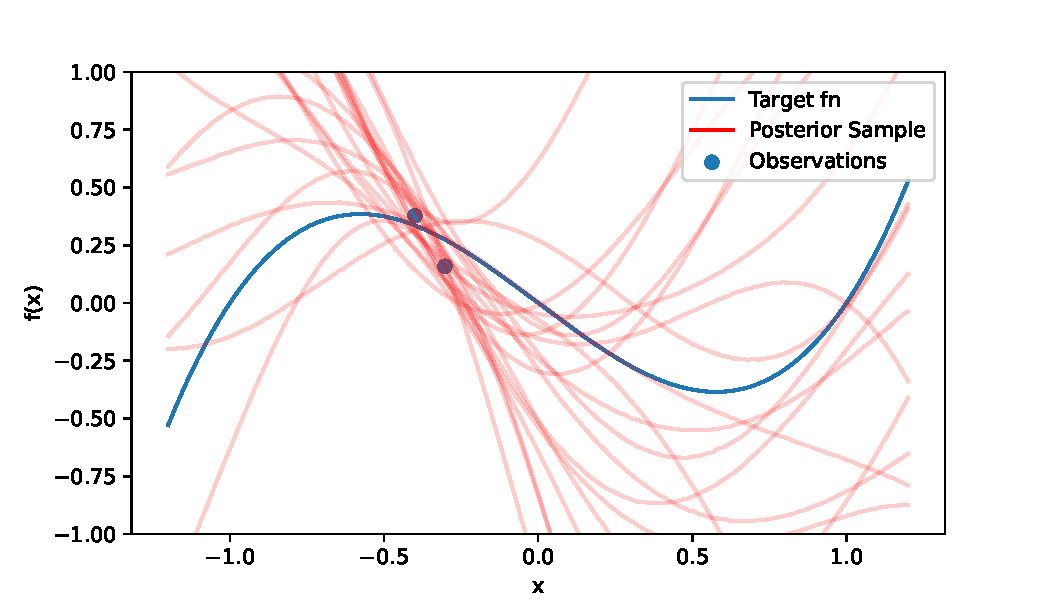
\includegraphics[width=\textwidth]{cub_GP_err_2_iters.pdf}
    \end{subfigure}%
    \hfill%
    \begin{subfigure}[b]{0.5\textwidth}
        \centering
        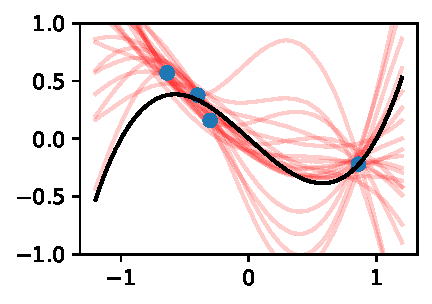
\includegraphics[width=\textwidth]{cub_GP_err_4_iters.pdf}
    \end{subfigure}
    \begin{subfigure}[b]{0.5\textwidth}
        \centering
        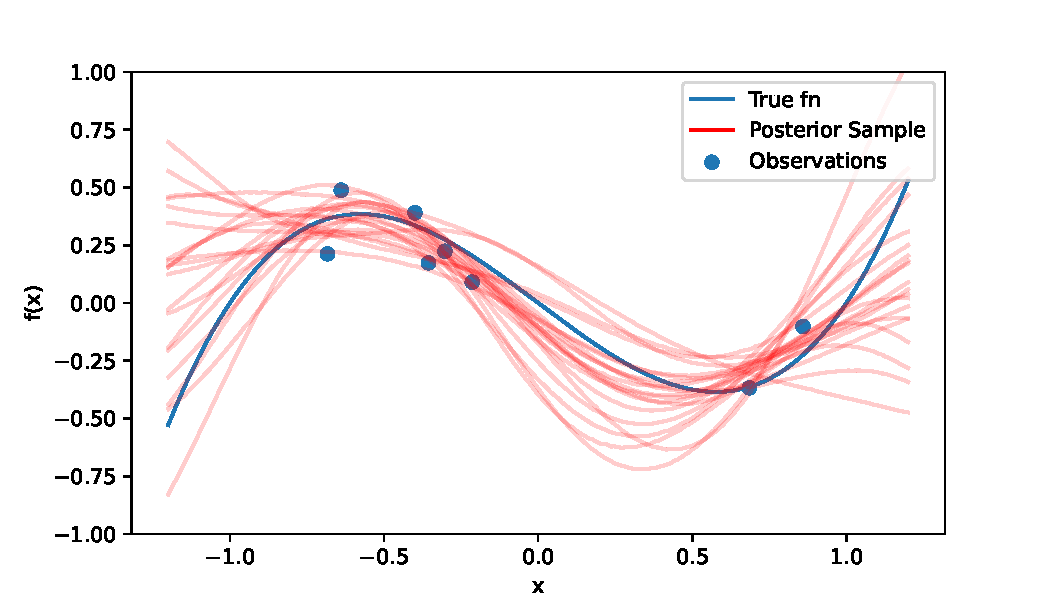
\includegraphics[width=\textwidth]{cub_GP_err_8_iters.pdf}
    \end{subfigure}%
    \hfill%
    \begin{subfigure}[b]{0.5\textwidth}
        \centering
        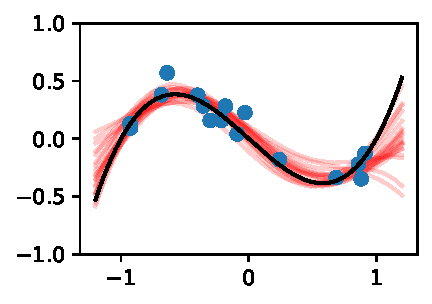
\includegraphics[width=\textwidth]{cub_GP_err_16_iters.pdf}
    \end{subfigure}%
    \caption{
        Sequence of Gaussian process regressions on the target function
        (black) $f(x) = x(x-1)(x+1),$ after 2, 4, 8, and 16 observations of
        $f(x_i) + \varepsilon_i,$ where $\varepsilon_i$ is i.i.d.\
        $\mathcal{N}(0, \sigma^2_o)$ with $\sigma^2_o = 0.01$
        in blue. The red lines are new realisations from the conditioned
        Gaussian process. The Gaussian process was 0 mean and had a squared
        exponential kernel. The hyperparameters were fixed with $\ell = 2.7$
        and $\sigma^2_k = 1.1$
    }
    \label{fig:var_cub_reg}
\end{figure}

Adding noise to the observations makes the Gaussian process regression
much less stable (Figure \ref{fig:var_cub_reg})

\subsection*{Model Selection}

A brief discussion of hyperparameter and mean function choice follows.
The hyperparameters $\ell$ and $\sigma^2_k$ for the choice of kernel have to be
fit, as they will not be known beforehand. There are two main ways to do this:
maximum likelihood estimation, and leave-one-out cross validation. 

\textcolor{red}{describe the two methods, look at ``Spline models for observational data"}

Recent work has shown that at least under specific conditions, the 
leave-one-out estimates for the scale parameter are more robust to a larger
class of target functions \parencite{naslidnyk_comparing_2024}, and the
broader literature seems


\section{Differing mean functions}



\begin{figure}[htbp]
    \missingfigure{GP mean functions}
\end{figure}

\section{Bayesian Acquisition Functions}

When considering Bayesian acquisition functions



\begin{itemize}
    \item Choosing the next point to sample
    \item $\argmin_{\bm{\theta}}A(\bm\theta)$ where A is an acquisition function.
    \item BOLFI paper uses $$\mu(\bm\theta) - \eta_t\sqrt{\mathrm{v}(\bm\theta)}$$ \begin{itemize}
              \item $\eta_t:= \sqrt{c + 2\ln(t^{d/2 + 2})},$ and $c$ can be chosen
              \item $\mu(\bm\theta)$ and $\mathrm{v}(\bm\theta)$ are the posterior mean and variance
          \end{itemize}

    \item Could use expected information
          $$
              (\mu_\text{min} - \mu(\bm\theta)) \varPhi \left(
              \frac{\mu_\text{min} - \mu(\bm\theta)}{\sqrt{\mathrm{v}(\bm\theta)}}
              \right)
              + \sqrt{\mathrm{v}(\bm\theta)}\phi\left(
              \frac{\mu_\text{min} - \mu(\bm\theta)}{\sqrt{\mathrm{v}(\bm\theta)}}
              \right)
          $$
          \begin{itemize}
              \item $\mu_\text{min} := \min_{\bm{\theta}} \mu(\bm\theta)$
              \item $\varPhi, \phi$ CDF and PDF of standard normal
          \end{itemize}
\end{itemize}
exploration parameter proven by \cite{srinivas_gaussian_2010}